\section{Laue-Aufnahme}\label{sec:laue}
In diesem Versuchsteil wird die Symmetrie und Gitterstruktur eine NaCl-Kristalls mithilfe des Laue-Verfahrens untersucht. Dabei wird der zu
untersuchende Kristall mit Röntgenstrahlung bestrahlt. Hinter dem Kristall ist ein Röntgenfilm platziert, auf dem die durch den Kristall laufende
Röntgenstrahlung nachgewiesen werden kann. Mithilfe des auf dem Röntgenfilm entstehenden Musters können dann einige Eigenschaften des verwendeten
Kristalls untersucht werden.
\subsection{Aufbau}\label{subsec:laue_aufbau}
Zur Durchführung dieses Versuchsteils wird der zu Verfügung stehende NaCl-Kristall verwendet. Die Röntgenstrahlung wird mit einer Molybdän-Röntgenröhre
erzeugt. Der Versuchsaufbau zur Laue-Aufnahme ist in \cref{fig:aufbau_laue} dargestellt.
\begin{figure}[H]
	\centering
	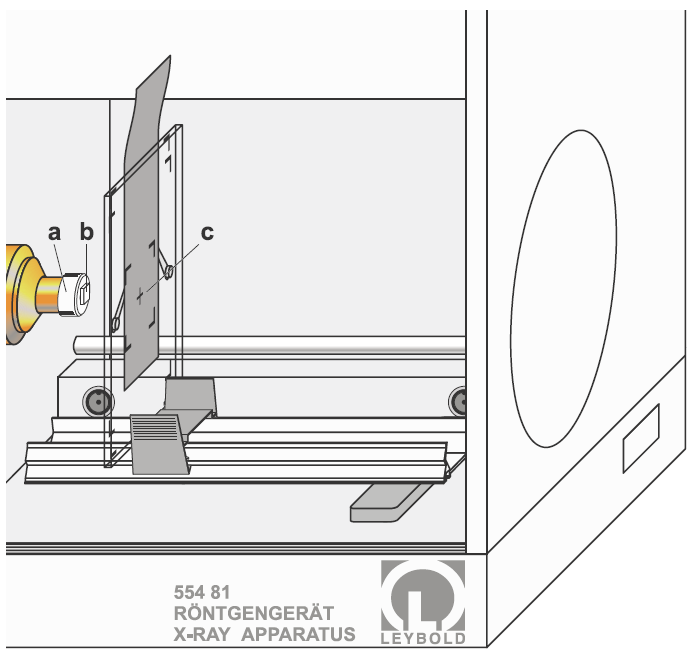
\includegraphics[width=0.6\linewidth]{../figs/aufbau_laue.png}
	\caption{Versuchsaufbau der Laue-Aufnahme zur Untersuchung eines NaCl-Kristalls \cite{laue_handblatt}.}
	\label{fig:aufbau_laue}
\end{figure} Zunächst wird die Molybdän-Röntgenröhre zur Erzeugung der benötigten Röntgenstrahlung eingesetzt. Aus dem Vollschutzröntgengerät werden Targethalter
und Sensorarm entfernt, sodass eine Experimentierschiene mittig vor die Kollimatoraufnahme platziert werden kann. In die Kollimatoraufnahme wird der Kollimator
mit \SI{1}{\milli \meter} Spaltbreite eingesetzt. Der verwendete NaCl-Kristall ist bereits auf einer Lochblende befestigt, welche deshalb sofort auf den Kollimator aufgesetzt
werden kann. Für die Laue-Aufnahme wird ein \textit{AGFA Dentus M2 Comfort} Röntgenfilm verwendet, welcher möglichst mittig auf der markierten Fläche
des Filmhalters festgeklemmt wird. Dabei muss darauf geachtet werden, dass der Film möglichst plan über seine gesamte Fläche aufliegt. Anschließend wird der Filmhalter
auf der Experimentierschiene platziert und verschoben, sodass zwischen NaCl-Kristall und Film ein Abstand von \SI{15(1)}{\milli \meter} (hier gibt es eine relativ große Unsicherheit,
da die Einstellung nicht allzu exakt vorgenommen werden konnte) eingestellt wird.\par
An dem Vollschutzröntgengerät wird eine Röhrenhochspannung von $U = \SI{35,0}{\kilo \volt}$ und ein Emissionsstrom von $I = \SI{1,0}{\milli \ampere}$ eingestellt.
Die Winkeländerung des Goniometers wird auf $\Delta \beta = \SI{0,0}{\degree}$ eingestellt. Schließlich wird die Messzeit auf $\Delta t = \SI{1800}{\second}$ eingestellt.
\subsection{Messung}\label{subsec:laue_messung}
\subsection{Auswertung}\label{subsec:laue_auswertung}
%\begin{table}[H]
%    \centering
%    \caption{Miller-Indizes}
%    \begin{tabular}{c|c|c|c|c|c|c|c}
%        Punkt & $x_{\mathrm{P}}'$ / p & $y_{\mathrm{P}}'$ / p & $x_{\mathrm{P}}$ / p & $y_{\mathrm{P}}$ / p & $z_{\mathrm{Q}}$ / p & $\Delta z_{\mathrm{Q}}$ / p & $(h,k,l)$ \\
%        \hline
%        A01 & 1289 & 1665 & -273 & -184 & 106 & 18 & $(\bar{5}\bar{3}2)$ \\
%        A02 & 1364 & 1660 & -198 & -189 &  75 & 14 & $(\bar{5}\bar{5}2)$ \\
%        A03 & 1360 & 1589 & -202 & -260 & 106 & 18 & $(\bar{3}\bar{5}2)$ \\
%        A04 & 1739 & 1538 &  177 & -311 & 123 & 20 & $(3\bar{5}2)$ \\
%        A05 & 1762 & 1623 &  200 & -226 &  90 & 16 & $(5\bar{5}2)$ \\
%        A06 & 1862 & 1623 &  300 & -226 & 134 & 21 & $(5\bar{3}2)$ \\
%        A07 & 1875 & 2058 &  313 &  209 & 134 & 21 & $(532)$ \\
%        A08 & 1776 & 2072 &  214 &  223 &  94 & 17 & $(552)$ \\
%        A09 & 1762 & 2158 &  200 &  309 & 129 & 21 & $(352)$ \\
%        A10 & 1363 & 2121 & -199 &  272 & 110 & 19 & $(\bar{3}52)$ \\
%        A11 & 1363 & 2030 & -199 &  181 &  73 & 14 & $(\bar{5}52)$ \\
%        A12 & 1283 & 2018 & -279 &  169 & 104 & 18 & $(\bar{5}32)$ \\
%        B01 & 1507 & 1638 &  -55 & -211 &  49 & 11 & $(\bar{1}\bar{4}1)$ \\
%        B02 & 1579 & 1623 &   17 & -226 &  53 & 11 & $(1\bar{4}1)$ \\
%        B03 & 1807 & 1793 &  245 &  -56 &  64 & 13 & $(4\bar{1}1)$ \\
%        B04 & 1810 & 1908 &  248 &   59 &  66 & 13 & $(411)$ \\
%        B05 & 1597 & 2086 &   35 &  237 &  59 & 12 & $(141)$ \\
%        B06 & 1507 & 2075 &  -55 &  226 &  55 & 12 & $(\bar{1}41)$ \\
%        B07 & 1360 & 1884 & -202 &   35 &  44 & 10 & $(\bar{4}11)$ \\
%        B08 & 1362 & 1803 & -200 &  -46 &  44 & 10 & $(\bar{4}\bar{4}1)$ \\
%        C01 & 1414 & 1482 & -148 & -367 & 147 & 23 & $(\bar{2}\bar{5}2)$ \\
%        C02 & 1535 & 1416 &  -27 & -433 & 172 & 25 & $(0\bar{5}2)$ \\
%        C03 & 1672 & 1450 &  110 & -399 & 159 & 24 & $(2\bar{5}2)$ \\
%        C04 & 1974 & 1695 &  412 & -154 & 176 & 26 & $(\bar{5}\bar{2}2)$ \\
%        C05 & 2039 & 1835 &  477 &  -14 & 203 & 28 & $(\bar{5}02)$ \\
%        C06 & 1983 & 1985 &  421 &  136 & 178 & 26 & $(522)$ \\
%        C07 & 1689 & 2248 &  127 &  399 & 162 & 24 & $(252)$ \\
%        C08 & 1548 & 2286 &  -14 &  437 & 175 & 26 & $(052)$ \\
%        C09 & 1422 & 2222 & -140 &  373 & 148 & 23 & $(\bar{2}52)$ \\
%        C10 & 1200 & 1958 & -362 &  109 & 135 & 22 & $(\bar{5}22)$ \\
%        C11 & 1161 & 1843 & -401 &   -6 & 150 & 23 & $(\bar{5}02)$ \\
%        C12 & 1205 & 1730 & -357 & -119 & 134 & 21 & $(\bar{5}\bar{2}2)$ \\
%        D01 & 1236 & 1543 & -326 & -306 & 181 & 26 & $(\bar{4}\bar{4}2)$ \\
%        D02 & 1891 & 1478 &  329 & -371 & 216 & 29 & $(4\bar{4}2)$ \\
%        D03 & 1913 & 2205 &  351 &  356 & 219 & 29 & $(442)$ \\
%        D04 & 1236 & 2152 & -326 &  303 & 180 & 26 & $(\bar{4}42)$ \\
%        E01 & 1025 & 1585 & -357 & -264 & 179 & 26 & $(\bar{4}\bar{2}2)$ \\
%        E02 & 1262 & 1302 & -300 & -547 & 315 & 36 & $(\bar{2}\bar{4}2)$ \\
%        E03 & 1830 & 1239 &  268 & -610 & 350 & 40 & $(2\bar{4}2)$ \\
%        E04 & 2175 & 1516 &  613 & -333 & 380 & 40 & $(4\bar{2}2)$ \\
%        E05 & 2204 & 2169 &  642 &  320 & 390 & 40 & $(422)$ \\
%        E06 & 1859 & 2462 &  297 &  613 & 360 & 40 & $(242)$ \\
%        E07 & 1262 & 2402 & -300 &  553 & 320 & 40 & $(\bar{2}42)$ \\
%        E08 & 1017 & 2104 & -545 &  255 & 300 & 40 & $(\bar{4}22)$ \\
%        F01 &  850 & 1390 & -712 & -459 & 500 & 50 & $(\bar{3}\bar{2}2)$ \\
%        F02 & 1057 & 1147 & -505 & -702 & 520 & 50 & $(\bar{2}\bar{3}2)$ \\
%        F03 & 2069 & 1016 &  507 & -833 & 620 & 50 & $(2\bar{3}2)$ \\
%        F04 & 2388 & 1260 &  826 & -589 & 650 & 50 & $(3\bar{2}2)$ \\
%        F05 & 2430 & 2431 &  868 &  582 & 680 & 50 & $(322)$ \\
%        F06 & 2115 & 2684 &  553 &  835 & 640 & 50 & $(232)$ \\
%        F07 & 1048 & 2583 & -514 &  734 & 540 & 50 & $(\bar{2}32)$ \\
%        F08 &  834 & 2309 & -728 &  460 & 520 & 50 & $(\bar{3}22)$                
%    \end{tabular}\label{tab:miller}
%\end{table}\newpage
\begin{table}[H]
    \centering
    \caption{Miller-Indizes}
    \begin{tabular}{c|c|c|c|c|c|c|c}
        Punkt & $x_{\mathrm{P}}'$ / p & $y_{\mathrm{P}}'$ / p & $x_{\mathrm{P}}$ / p & $y_{\mathrm{P}}$ / p & $z_{\mathrm{Q}}$ / p & $\Delta z_{\mathrm{Q}}$ / p & $(hkl)$ \\
        \hline
        A01 & $1289$ & $1665$ & $-273$ & $-184$ & $ 81$ & $13$ & $(\bar{3}\bar{2}1)$ \\
        A02 & $1364$ & $1660$ & $-198$ & $-189$ & $ 57$ & $10$ & $(\bar{3}\bar{3}1)$ \\
        A03 & $1360$ & $1589$ & $-202$ & $-260$ & $ 81$ & $13$ & $(\bar{2}\bar{3}1)$ \\
        A04 & $1739$ & $1538$ & $ 177$ & $-311$ & $ 95$ & $14$ & $(2\bar{3}1)$ \\
        A05 & $1762$ & $1623$ & $ 200$ & $-226$ & $ 69$ & $11$ & $(3\bar{3}1)$ \\
        A06 & $1862$ & $1623$ & $ 300$ & $-226$ & $104$ & $15$ & $(3\bar{2}1)$ \\
        A07 & $1875$ & $2058$ & $ 313$ & $ 209$ & $104$ & $15$ & $(321)$ \\
        A08 & $1776$ & $2072$ & $ 214$ & $ 223$ & $ 72$ & $12$ & $(331)$ \\
        A09 & $1762$ & $2158$ & $ 200$ & $ 309$ & $100$ & $14$ & $(231)$ \\
        A10 & $1363$ & $2121$ & $-199$ & $ 272$ & $ 85$ & $13$ & $(\bar{2}31)$ \\
        A11 & $1363$ & $2030$ & $-199$ & $ 181$ & $ 55$ & $10$ & $(\bar{3}31)$ \\
        A12 & $1283$ & $2018$ & $-279$ & $ 169$ & $ 80$ & $13$ & $(\bar{3}21)$ \\
        B01 & $1507$ & $1638$ & $ -55$ & $-211$ & $ 37$ & $ 7$ & $(\bar{1}\bar{6}1)$ \\
        B02 & $1579$ & $1623$ & $  17$ & $-226$ & $ 40$ & $ 7$ & $(1\bar{6}1)$ \\
        B03 & $1807$ & $1793$ & $ 245$ & $ -56$ & $ 48$ & $10$ & $(6\bar{1}1)$ \\
        B04 & $1810$ & $1908$ & $ 248$ & $  59$ & $ 50$ & $10$ & $(611)$ \\
        B05 & $1597$ & $2086$ & $  35$ & $ 237$ & $ 44$ & $ 8$ & $(161)$ \\
        B06 & $1507$ & $2075$ & $ -55$ & $ 226$ & $ 42$ & $ 8$ & $(\bar{1}61)$ \\
        B07 & $1360$ & $1884$ & $-202$ & $  35$ & $ 33$ & $ 8$ & $(\bar{6}11)$ \\
        B08 & $1362$ & $1803$ & $-200$ & $ -46$ & $ 33$ & $ 8$ & $(\bar{6}\bar{1}1)$ \\
        C01 & $1414$ & $1482$ & $-148$ & $-367$ & $114$ & $16$ & $(\bar{1}\bar{3}1)$ \\
        C02 & $1535$ & $1416$ & $ -27$ & $-433$ & $135$ & $17$ & $(0\bar{3}1)$ \\
        C03 & $1672$ & $1450$ & $ 110$ & $-399$ & $124$ & $16$ & $(1\bar{3}1)$ \\
        C04 & $1974$ & $1695$ & $ 412$ & $-154$ & $139$ & $18$ & $(3\bar{1}1)$ \\
        C05 & $2039$ & $1835$ & $ 477$ & $ -14$ & $161$ & $20$ & $(301)$ \\
        C06 & $1983$ & $1985$ & $ 421$ & $ 136$ & $140$ & $19$ & $(311)$ \\
        C07 & $1689$ & $2248$ & $ 127$ & $ 399$ & $127$ & $17$ & $(131)$ \\
        C08 & $1548$ & $2286$ & $ -14$ & $ 437$ & $137$ & $18$ & $(031)$ \\
        C09 & $1422$ & $2222$ & $-140$ & $ 373$ & $116$ & $16$ & $(\bar{1}31)$ \\
        C10 & $1200$ & $1958$ & $-362$ & $ 109$ & $105$ & $15$ & $(\bar{3}11)$ \\
        C11 & $1161$ & $1843$ & $-401$ & $  -6$ & $117$ & $17$ & $(\bar{3}01)$ \\
        C12 & $1205$ & $1730$ & $-357$ & $-119$ & $104$ & $15$ & $(\bar{3}\bar{1}1)$ \\
        D01 & $1236$ & $1543$ & $-326$ & $-306$ & $143$ & $19$ & $(\bar{2}\bar{2}1)$ \\
        D02 & $1891$ & $1478$ & $ 329$ & $-371$ & $172$ & $21$ & $(2\bar{2}1)$ \\
        D03 & $1913$ & $2205$ & $ 351$ & $ 356$ & $175$ & $21$ & $(221)$ \\
        D04 & $1236$ & $2152$ & $-326$ & $ 303$ & $142$ & $18$ & $(\bar{2}21)$ \\
        E01 & $1025$ & $1585$ & $-357$ & $-264$ & $141$ & $18$ & $(\bar{2}\bar{1}1)$ \\
        E02 & $1262$ & $1302$ & $-300$ & $-547$ & $257$ & $27$ & $(\bar{1}\bar{2}1)$ \\
        E03 & $1830$ & $1239$ & $ 268$ & $-610$ & $288$ & $29$ & $(1\bar{2}1)$ \\
        E04 & $2175$ & $1516$ & $ 613$ & $-333$ & $310$ & $30$ & $(2\bar{1}1)$ \\
        E05 & $2204$ & $2169$ & $ 642$ & $ 320$ & $330$ & $30$ & $(211)$ \\
        E06 & $1859$ & $2462$ & $ 297$ & $ 613$ & $300$ & $30$ & $(121)$ \\
        E07 & $1262$ & $2402$ & $-300$ & $ 553$ & $261$ & $27$ & $(\bar{1}21)$ \\
        E08 & $1017$ & $2104$ & $-545$ & $ 255$ & $242$ & $26$ & $(\bar{2}11)$ \\
        F01 & $ 850$ & $1390$ & $-712$ & $-459$ & $430$ & $40$ & $(\bar{3}\bar{2}2)$ \\
        F02 & $1057$ & $1147$ & $-505$ & $-702$ & $440$ & $40$ & $(\bar{2}\bar{3}2)$ \\
        F03 & $2069$ & $1016$ & $ 507$ & $-833$ & $530$ & $50$ & $(2\bar{3}2)$ \\
        F04 & $2388$ & $1260$ & $ 826$ & $-589$ & $570$ & $50$ & $(3\bar{2}2)$ \\
        F05 & $2430$ & $2431$ & $ 868$ & $ 582$ & $590$ & $50$ & $(322)$ \\
        F06 & $2115$ & $2684$ & $ 553$ & $ 835$ & $550$ & $50$ & $(232)$ \\
        F07 & $1048$ & $2583$ & $-514$ & $ 734$ & $470$ & $40$ & $(\bar{2}32)$ \\
        F08 & $ 834$ & $2309$ & $-728$ & $ 460$ & $440$ & $40$ & $(\bar{3}22)$                
    \end{tabular}\label{tab:miller2}
\end{table}